%%=============================================================================
%% Methodologie
%%=============================================================================

\chapter{\IfLanguageName{dutch}{Methodologie}{Methodology}}
\label{ch:methodologie}

%% TODO: Hoe ben je te werk gegaan? Verdeel je onderzoek in grote fasen, en
%% licht in elke fase toe welke stappen je gevolgd hebt. Verantwoord waarom je
%% op deze manier te werk gegaan bent. Je moet kunnen aantonen dat je de best
%% mogelijke manier toegepast hebt om een antwoord te vinden op de
%% onderzoeksvraag.

In de vorige hoofdstukken werden de frameworks die in deze studie vergeleken zullen worden geselecteerd en hun achtergrond besproken. In dit hoofstuk wordt de effectieve vergelijking tussen de verschillende frameworks gemaakt. Er wordt gestart met een vergelijking over de manier waarop de verschillende frameworks bepaalde zaken zoals o.a. het navigeren tussen verschillende pagina's van een app aanpakken. Vervolgens wordt er een prestatievergelijking gemaakt aan de hand van een applicatie die op alle drie de frameworks geschreven wordt. 

\section{Vergelijking eigenschappen}
\label{sec:vglEigenschappen}

Elk framework heeft zijn eigen manier om bepaalde zaken aan te pakken. In deze sectie worden de verschillende aanpakken van de frameworks besproken op het gebied van navigatie, toegang tot de native API's, opbouwen van de gebruikersinterface van de applicatie en de styling van de applicatie.

\subsection{Navigatie binnen de applicatie}
\label{subsec:navigatieApplicatie}

Een belangrijk deel van elke applicatie is de mogelijkheid om te kunnen navigeren tussen verschillende pagina's van de applicatie. Elk cross-platform framework moet dus de mogelijkheid voorzien om de ontwikkelaar toe te staan deze functionaliteit te verwerken in de applicatie. Elk framework gaat hier op zijn eigen manier mee om en in deze sectie worden de verschillende aanpakken van de drie gekozen frameworks besproken.

\subsubsection{React Native}
\label{subsubsec:navigatieReactNative}

React Native maakt voor de navigatie tussen de verschillende pagina's gebruik van een library genaamd React Native Navigation. Dit is een stand-alone library die de ontwikkelaar in staat stelt om zowel op Android als iOS navigatie aan te leveren die een native uitstraling heeft. Het is één van de vele populaire libraries binnen React Native die ontwikkeld zijn door de uitgebreide community achter React Native. Onderliggend maakt deze library ook gebruik van een andere library genaamd Animated om de animaties tijdens het navigeren naar een andere pagina aan te bieden. De animaties en gebaren die gepaard gaan met het navigeren kunnen volledig aangepast worden aan de voorkeuren van de ontwikkelaar. Er is dus zeer veel vrijheid en de gebruiker krijgt een applicatie die navigeert zoals een native applicatie. 

Om de navigatie te gebruiken moet de ontwikkelaar de hele applicatie wrappen in een navigatiecontainer. Op deze manier heeft de library toegang tot de gehele applicatie en kan de ontwikkelaar de navigatie tussen de verschillende pagina's instellen naar wens. De werkwijze om de applicatie te wrappen met de navigatiecontainer en de verschillende pagina's toe te voegen aan de navigatiestack is te zien in figuur \ref{fig:opzettenNavigatieReactNative}.

\begin{figure}
    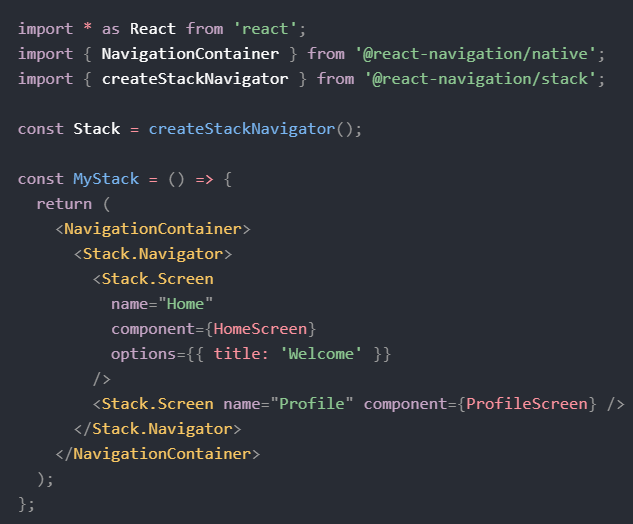
\includegraphics[width=\linewidth]{OpzettenNavigatieReactNative.png}
    \caption{Opzetten navigatie in een React Native applicatie. Bron: reactnative.dev/docs/navigation}
    \label{fig:opzettenNavigatieReactNative}
\end{figure}

Vervolgens moet er vastgelegd worden naar welke pagina er genavigeerd moet worden bij de uitvoering van een bepaald actie, zoals bv de klik op een bepaalde knop. Om dit mogelijk te maken krijgt elke component die een pagina voorsteld een attribuut navigation mee. In dit attribuut zitten methodes van de library die het navigeren tussen de verschillende pagina's mogelijk maakt. De opzet van een simpele navigatie is te zien in figuur \ref{fig:navigerenReactNative}. 

Zoals eerder vermeld heeft de library zeer veel mogelijkheden en levert het een navigatie af die native aanvoelt voor de gebruiker. Om dit te bereiken beschikt React Native Navigation ook over verschillende packages die o.a. tabs en drawer functionaliteit aanbieden. Dit zijn twee populaire manieren om te navigeren binnen een applicatie. Door dit aan te bieden in een package moet de ontwikkelaar niet helemaal zelf deze funtionaliteit gaan uitwerken en wordt de standaard die de gebruiker gewoon is van native applicaties geëvenaard.

\begin{figure}
    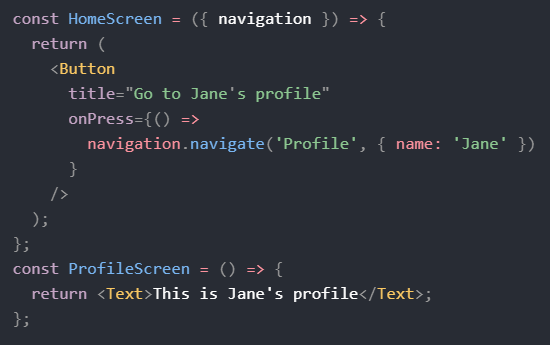
\includegraphics[width=\linewidth]{NavigerenPaginasReactNative.png}
    \caption{Navigeren naar een andere pagina in React Native. Bron: reactnative.dev/docs/navigation}
    \label{fig:navigerenReactNative}
\end{figure}



